\pdfminorversion=4
\documentclass[notes=hide]{beamer}
%\includeonlyframes{results}
\usepackage[overlay,absolute]{textpos}
\usepackage{natbib,tikz}
\tikzstyle{every picture}+=[remember picture]
\tikzstyle{na} = [baseline=-.5ex]
\setlength{\TPHorizModule}{\paperwidth}
\setlength{\TPVertModule}{\paperheight}
\definecolor{UniGray}{RGB}{94, 94, 87}
\definecolor{UniRed}{RGB}{90, 0, 20}
\setbeamercolor{alert}{fg=red}
\setbeamercolor{block title}{bg=white}
\setbeamercolor{block body}{bg=white}
\newcommand{\mpoint}[1]{
  {\usebeamercolor[fg]{alert}#1}
}
\setbeamerfont{small}{size=\scriptsize}
{
\mode<presentation>
{
  \usetheme[footheight=0.3cm]{boxes}
  \addfootboxtemplate{\color{UniGray}}{\hspace{0.0cm}
    \color{white}
    
\includegraphics[height=0.8cm]{IUP-Logo.pdf}
    \hspace{2cm}
    Mathias Palm 
    \hfill
    \hspace{2cm}
%    \includegraphics[height=0.8cm]{RAM-Logo.eps}
%    \hfill\color{white}\insertshorttitle\hfill
%    \insertshortauthor
    \insertframenumber / \inserttotalframenumber
    \hfill
  } 
  % or ...

  \setbeamercovered{transparent=0}
}

\beamertemplatenavigationsymbolsempty

\usepackage[english]{babel}
\usepackage[latin1]{inputenc}
\usepackage{graphicx, colortbl}
\usepackage{times}
\usepackage[T1]{fontenc}

% \defbeamertemplate{background}{world-ndacc}
% {
% \includegraphics[height=\paperheight,width=\paperwidth]{ftir_ndacc.pdf}
% }


\title {SFIT4 -- Quickstart HOWTO}

\author[Mathias Palm]{Mathias Palm} 


\date{Bremen, 2020}

\begin{document}

\begin{frame}
\maketitle
\end{frame}

\begin{frame}
  \frametitle{Introduction}
  \framesubtitle{Absorption spectroscopy}
  \begin{columns}
    \begin{column}[t]{0.5\textwidth}
      \vspace{-1cm}
      \begin{figure}[!h]
        \centering
        \includegraphics<1->[scale=0.5]{Spectro_Principle_Atm.pdf}
        \label{fig:meas_principle}
      \end{figure}
      Measurements in solar or lunar absorption and emission possible 
    \end{column}
    \begin{column}[t]{0.5\textwidth}
      \uncover<2->{

        Received spectrum given by the sum of all absorption along the
        path of sight.}
        \begin{overlayarea}{\textwidth}{0.7\textheight}
          \only<2>{
            \includegraphics<2>[width=\textwidth]{meas_spec_3900_4400.pdf}
            
            Envelope defined by band filter 3900 - 4400 $cm^{-1}$
            }
          \only<3>{
          \includegraphics<3>[width=\textwidth]{meas_spec_4235_4236.pdf}
          
          Microwindow containing a CO-line
          }
          \only<4>{
            \includegraphics<4>[width=\textwidth,height=0.4\textheight]{CO_main_gases.pdf}

            Contribution of gases and solar lines not calculated for
            this particular spectrum
            }
        \end{overlayarea}
      \end{column}
  \end{columns}
\end{frame}

\begin{frame}
  \frametitle{Introduction}
  \framesubtitle{Principle of a Fourier transform spectrometer}
  \begin{columns}
    \begin{column}{0.6\textwidth}
      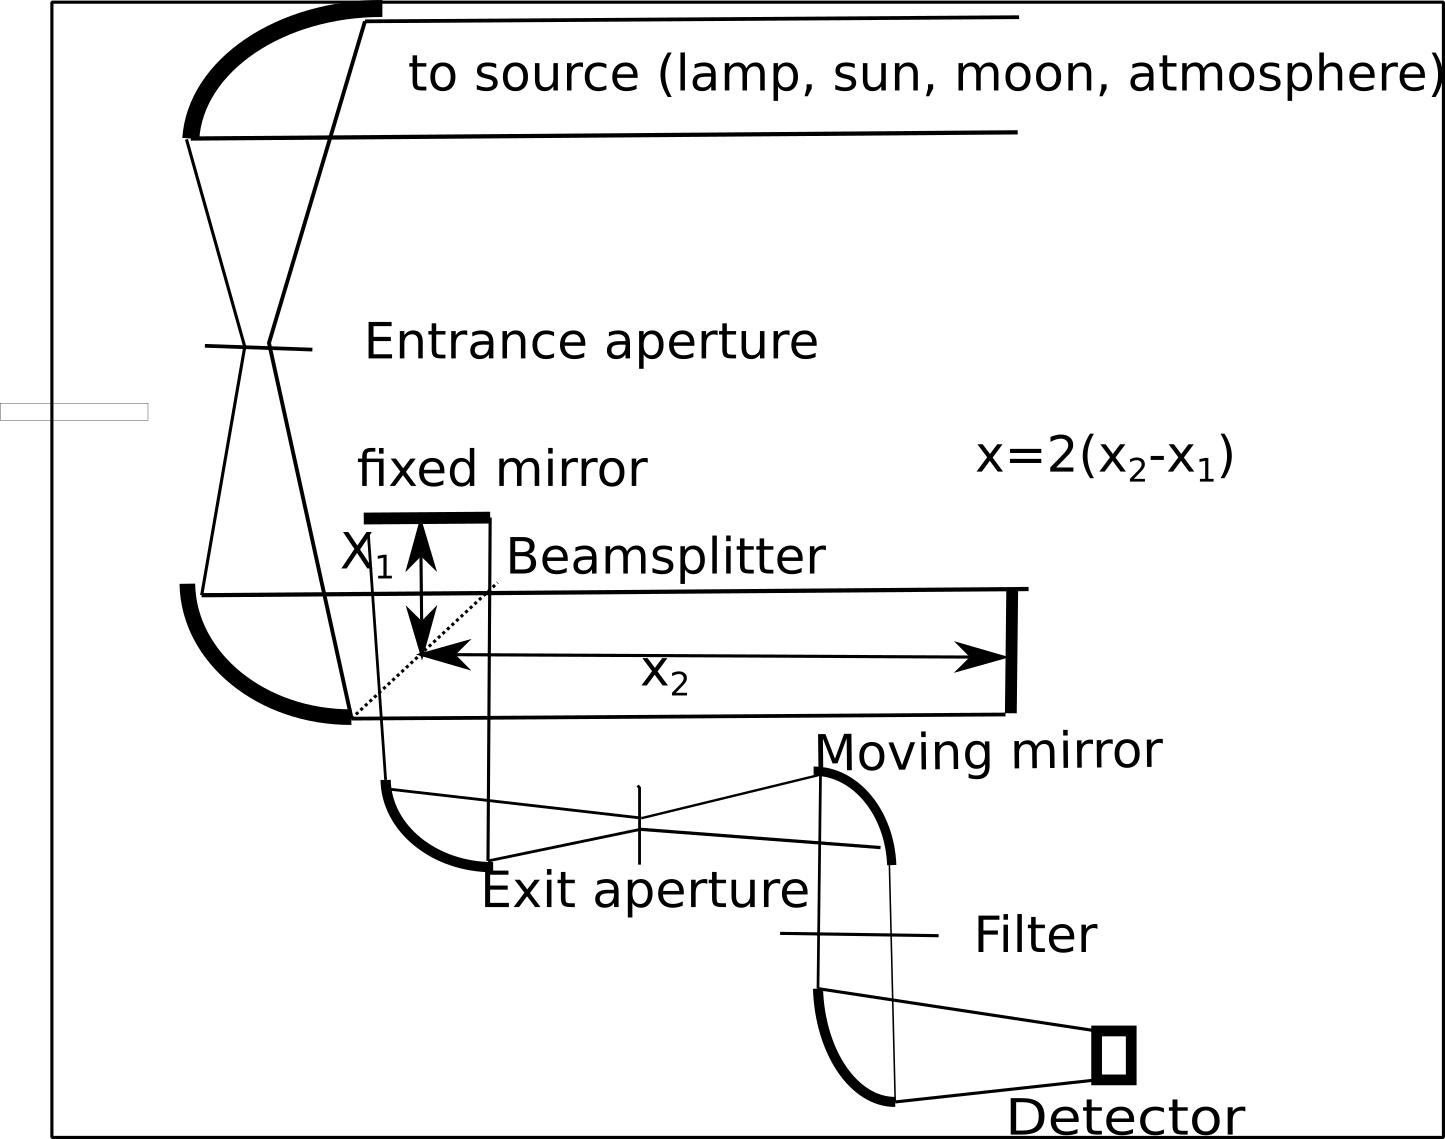
\includegraphics[width=1.2\textwidth,height=0.8\textheight]{Principle-fts.png}
    \end{column}
    \begin{column}{0.4\textwidth}
      \vspace{-2cm}
      \begin{itemize}
      \item apertures define and restrict field of view
      \item aperture influences resolution
      \item filter restricts wavelength sensitivity
      \end{itemize}
     \end{column}
    \end{columns}
\end{frame}


\begin{frame}
  \frametitle{Contents}
  \begin{itemize}
  \item Other documentation files and what they contain
  \item Files needed and where to get them
  \item How to modify sfit4.ctl
  \item Create the spectral file LLLLL.llllll-HHHHH.hhhhhh.hbin
  \item Run SFIT4
  \end{itemize}
\end{frame}

\begin{frame}
  \frametitle{Other descritions and what they contain}
  \begin{description}
  \item[sfit4\_init/sfit4\_init.pdf] The tentative description of the
    keys in the sfit4.ctl file and their interdependencies
  \item[hbin/sfit4-hbin\_ctl.docx] describes the structure of the
    hbin.ctl file (input file of hbin) to create the file
    LLLLL.llllll-HHHHH.hhhhhh.hbin
  \item[Linelist/sfit4-isotope\_descrip.docx] contains the structure of
    the file.in.isotope file 
  \item[Linelist/sfit4-isotope\_descrip.docx] contains the structure of
    the file.in.isotope file 
  \item[ForwardModel/sfit4-lineshapes.pdf] summarizes the lineshape options available in SFIT4.
  \item[ForwardModel/Workshop2019-Palm-sfit4-fwdmodel-params.pdf] contains many
    descriptions of forward model parameters. Is refered to as FWDMODEL-PARAMS.
  \end{description}
\end{frame}



\begin{frame}
  \frametitle{Files needed and where to get them}
  \framesubtitle{Files always necessary}
  The section file.in
  contains the names of the input files. The structure of the files is
  described on extra slides later on.
  \begin{description}
  \item[file.in.spectrum] The measured spectrum. This file is created
    using pspec or any other tool. Is also needed for calclating a
    synthetic spectrum, because it defines the spectral grid, SFIT4 is
    working on.
  \item[file.in.stalayers] The file containing the altitude bins for
    the forward model and the retrieval. This file defines the
    altitude grid which is used in SFIT4.
  \item[file.in.refprofile] Contains the atmosphere and is created by
    the processing environment or elsewhere. The atmosphere used in
    SFTI4 is interpolated to the altitudes given in file.in.stalayers,
    i.e. its range has to be equal or larger
  \item[LLLLL.llllll-HHHHH.hhhhhh.hbin] Contains the spectral data and
    is created by hbin (part of the sfit4 package, check sfit4-hbin\_ctl.docx)
  \end{description}
\end{frame}

\begin{frame}
  \frametitle{Files needed and where to get them}
  \framesubtitle{Files needed for certain optional calculations}
  \begin{description}
  \item[file.in.solarlines] needed is fw.solarspectrum = T. Is a
    linelist of solar lines and part of the spectroscopy which comes
    with SFIT4
  \item[file.in.modulation\_fcn] needed is fw.apod\_fcn =
    T. Parameters of the empirical apodisation function. See file
    FWDMODEL\_PARAMS slide 3ff.
  \item[file.in.phase\_fcn] needed if fw.phase\_fcn = T, Parameters of
    empirical phase function. See file
    FWDMODEL\_PARAMS slide 3ff. 
  \item[file.in.isotope] needed if fw.isotope\_separation =
    T. Contains definitions necessary for treating isotopes separetly
    from the main isotope of the retrieved gas. Check the file
    sfit4-isotope\_descrip.docx for its structure and
    contents. Files for the most common isotopes are part of the
    spectroscopy which comes with SFIT4.
  \end{description}
\end{frame}

\begin{frame}
  \frametitle{Download and build SFIT4, HBIN and PSPEC}
  From <https://wiki.ucar.edu/display/sfit4/->SFIT 4 Version 1.0.+
  (Pre) Release> download the following files:
  \begin{description}
  \item [sfit4\_v1.0.zip] contains the sfit4, hbin and pspec programs
  \item[linelist-core-20200706.tar.gz]  contains the linelist which
    are used with SFIT4
  \end{description}
  \begin{enumerate}
  \item unpack both archives
  \item in the directory sfit-core-code/src: type\\
    make clean\\
    make\\
    SFIT4 has been tested with gfortran version 9.3.0. Most of the
    gfortran builds work, but we would recomment to use at least
    gfortran version 8.0.
  \item go into directory sfit-core-code/sfit4\_testbed, modify
    test.cfg and run\\
    python2.7 script/run\_testcases.py\\
    If test.cfg is still filled in with the place-holders it will ask
    for the directories. Details are found in the README file.
  \end{enumerate}
\end{frame}

\begin{frame}
  \frametitle{Download and build SFIT4, HBIN and PSPEC (cont'd)}
  \begin{enumerate}
    \setcounter{enumi}{3}
  \item After it finishes it compares the results to the results
    stored in sfit4\_testbed/results\_v1.0 and prints out the differences
    if they are any. The differences should be small (fractions of a
    percent) if not, use another compiler.
  \item in the hbin.ctl set the key\\
    file.in.linelist\\
    to your linelist directory.
  \item run some or all of the testcases in test\_cases\_NDACC. It is
    better you start modifying testcases rather than building up a new
    one from scratch.
  \end{enumerate}
\end{frame}


\begin{frame}
  \frametitle{Getting help}
  \begin{enumerate}
  \item make sure you have the latest SFIT4 version (check on <https://wiki.ucar.edu/display/sfit4/>)
  \item Pack a full testcase, i.e.
    \begin{enumerate}
    \item sfit4.ctl
    \item hbin.ctl
    \item all files the section file.in. point to
    \item sfit4.dtl if it exists.
    \item a screenshot of the output.
    \end{enumerate}
  \item sent them to one or all people listet in the CONTACT section
    of <https://wiki.ucar.edu/display/sfit4/>.
  \item We rely on bug reports to improve the program further. Many
    bugs tend to be subtle and turn up only in very special
    circumstances.
  \end{enumerate}

\end{frame}
\end{document}
